%n LaBAC (see Figure \ref{fig:labac-model}), we have one attribute assigned to objects and one attribute assigned to users. Object attribute is named  \emph{object-label} and user attribute is named \emph{user-label}. These attributes are set valued attributes and the values of the attributes may form a partial order. 
%Note that, both object-label and user-label are a special type of attribute  which we do not elaborate here for brevity.

\emph{Object and Object-label}: Object is any resource we want to protect, for example, a JSON document, a JSON object or a XML tag. Object-label is a set valued attribute assigned on the objects. The values of this attribute may form a partial order.

%\emph{Object-label}: Object-label is the attribute assigned on the objects. The values of this attribute  form a partial order.

\emph{User} and \emph{user-label}: User-label is a set valued attribute assigned on users. Values of this attribute  may form a partial order. In a simple case, user-label values can be the set of roles assigned to the user. 

\emph{Action}: \textit{Action} is the set of available actions.


\emph{Policy}: A policy in this model is a tuple of (\emph{user-label}, \emph{action},  \emph{object-label}). The policy is interpreted such that objects labeled with any of \textit{object-label} values are allowed to be accessed by the users labeled with any of  \textit{user-label} values for the specific \textit{action}.


\emph{Attribute Hierarchy}: Using attribute hierarchy (Fig. \ref{fig:attribute-hierarchy}), if a policy allows an action for user-label $l_{uj}$ on object-label $l_{oj}$, all users having a equivalent or senior label than $l_{uj}$ can also access object-label $l_{oj}$ or its junior labels.

\begin{figure}
  \centering
    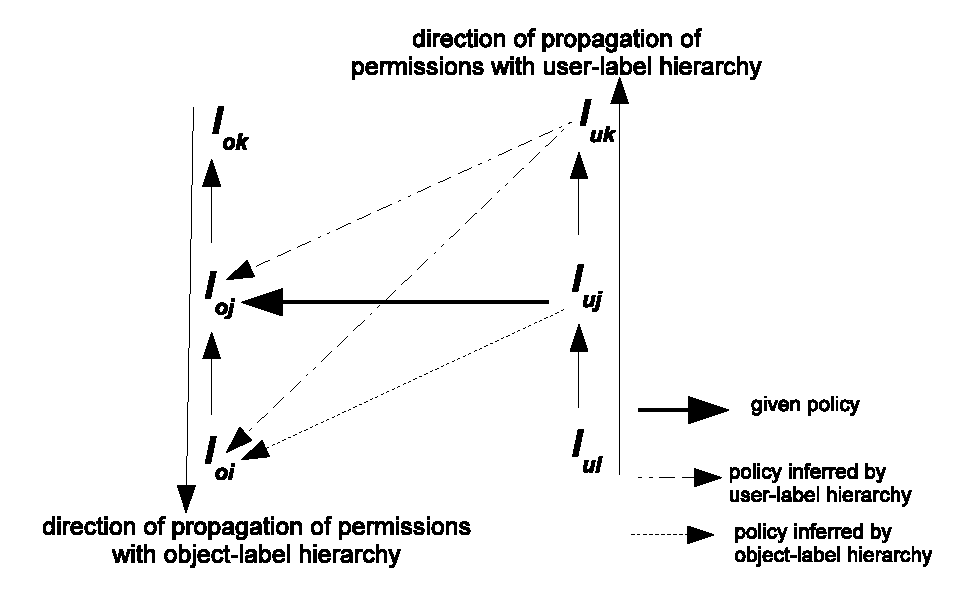
\includegraphics[width=0.5\textwidth]{attribute-hierarchy.eps}
 \caption{Propagation of permission with attribute hierarchy.}
 \label{fig:attribute-hierarchy}
\end{figure}

%\emph{Configuration points}: In the model, it is not specified how to assign object-labels on objects and user-labels on users. While, roles can be considered as user-labels, and user-role assignment problem is well studied, we only consider object, object-label assignment problem in our following discussion. 

%===================Policy Configuration starts ==================%
\begin{table*}[t] \footnotesize
	\centering
	\caption{LaBAC - Formal Definition}
	\label{table:labac-formal-model}
	\begin{tabular}{p{\textwidth}}
		
		\hline
		\textbf{Basic sets:}\\
		
		O = finite set of existing objects \\
		OL = finite set of object-label values\\
		A = finite set of actions\\
		U = finite set of existing users\\
		UL = finite set of user-label values\\
		
		\textbf{Basic functions and relations:}\\
		
		\emph{object-label}: $O \rightarrow 2^{OL} $ is a function mapping an object $o_{i}$ $\in$ O to a set of object-label values object-label($o_{i}$)\\
		
		\emph{user-label}: $U \rightarrow 2^{UL} $ is a function mapping an user $u_{i}$ $\in$ U to a set of uer-label values user-label($u_{i}$)\\
		
		\emph{objects}: $OL \rightarrow 2^ {O}$ is a function, given $ l \in OL $, it returns a set of objects which have been assigned label $l$. $objects(l) \equiv \left\{   o | \forall  o \in O, l \in object-label(o)       \right\}$ \\
		
		\emph{users}: $UL \rightarrow 2^ {U}$ is a function, given $ l \in UL $, it returns  a set of users which have been assigned label $l$. $users(l) \equiv \left\{   u | \forall  u \in U, l \in user-label(u)       \right\}$ \\
		
		\emph{allow}: $OL \times A \times UL \rightarrow \left\{true, false \right\}$ is a function defined over $l_{o} \in OL$ , $a \in A$ and $l_{u} \in U$ which returns \emph{true} if all users of  $users(l_{u})$ are allowed to exercise action $a$ on all objects of $objects(l_{o})$ \\
		
		\emph{$policy_{x}$} $ \subseteq OL \times A \times UL$ and for each tuple( $l_{o}, a_{i}, l_{u}$ ) $\in$ P, allow(  $l_{o}, a_{i}, l_{u}$ ) is true. [without hierarchy] \\
		
		\emph{$policy_{o}$} $ \subseteq OL \times A \times UL$ and for each tuple( $l_{oj}, a_{i}, l_{u}$ ) $\in$ P, allow(  $l_{ok}, a_{i}, l_{u}$ ) is true where $l_{oj} \ge l_{ok}$. [with object-label hierarchy] \\
		
		\emph{$policy_{u}$} $ \subseteq OL \times A \times UL$ and for each tuple( $l_{o}, a_{i}, l_{uj}$ ) $\in$ P, allow(  $l_{o}, a_{i}, l_{uk}$ ) is true where $l_{uk} \ge l_{uj}$. [with user-label hierarchy] \\
		
		\emph{policy} $ \subseteq OL \times A \times UL$ and for each tuple( $l_{oj}, a_{i}, l_{uj}$ ) $\in$ P, allow(  $l_{ok}, a_{i}, l_{uk}$ ) is true where $l_{oj} \ge l_{ok}$ and $l_{uk} \ge l_{uj}$. [with both of object-label and user-label hierarchy] \\
		
		\hline
	\end{tabular}
\end{table*}
